\documentclass[11pt,letterpaper]{article}

%\usepackage{times}
%\usepackage{epsfig}
\usepackage{graphicx}
%\usepackage{amsmath}
%\usepackage{amssymb}
\usepackage{hyperref}
\usepackage{tabularx}
\usepackage[left=1in, right=1in, top=1in, bottom=1in]{geometry}
\usepackage{titling}
\usepackage{setspace}
\usepackage{sectsty}
\usepackage{tabto}
\graphicspath{{./Assignment_02_NOTEBOOK_Geidel_files/}} % adds the assets directory to the path, throw your images there
\usepackage{fancyhdr}
\pagestyle{fancy}
\fancyhf{}
\fancyheadoffset{0cm}
\renewcommand{\headrulewidth}{0pt} 
\renewcommand{\footrulewidth}{0pt}
\fancyhead[R]{\thepage}
\fancypagestyle{plain}{%
  \fancyhf{}%
  \fancyhead[R]{\thepage}%
}

\usepackage{cite}
\usepackage[sectionbib]{natbib}
\renewcommand{\refname}{}

\begin{document}
\fontfamily{ptm}\selectfont
\sectionfont{\fontsize{12}{12}\fontfamily{ptm}\selectfont}
\doublespacing
%%%%%%%%%%%%%%%%%%%%%%%%%%%%%% TITLE %%%%%%%%%%%%%%%%%%%%%%%%%%%%%%%%%%%%%%
\setlength{\droptitle}{1in} 

\title{\large{ASSIGNMENT 2: \\ SALES RECOMMENDATION AGENT \\\vspace{1.2in}}}

\author{
Kevin Geidel \\
MSDS 442: AI Agent Design \& Development \\
Northwestern University \\
May 11, 2025 \\
}

\date{}
\maketitle
\thispagestyle{empty}	
\clearpage
\setcounter{page}{1}

%%%%%%%%%%%%%%%%%%%%%%%%%%%%%% PAGE 1 %%%%%%%%%%%%%%%%%%%%%%%%%%%%%%%%%%%%

\section*{Requirement 1: Graph the Agent with LangChain/LangGraph}
    \tab The construction of the agent and accompanying graph begins in cell 2 (see appendix). 
    The actual assembly of the graph occurs in cell 5. However, some of the components, such as the retriever \textbf{ToolNode} and \textbf{AgentState} class,
    are built above. Following the logic in cell 5 we first instantiate an empty graph:

    \begin{verbatim}
    workflow = StateGraph(AgentState)
    \end{verbatim}

    The \texttt{workflow} object has \texttt{add\_node} and \texttt{add\_edge} methods that allow us to assemble the 
    components created in cells 2-6. The output is displayed graphically in cell 6 (reproduced below.)
    \begin{center}
        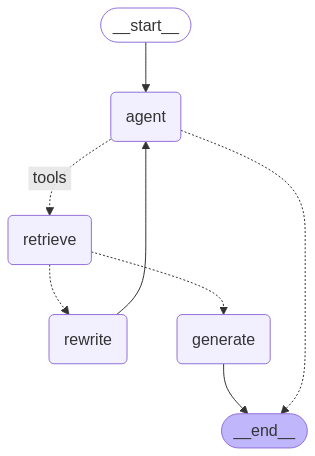
\includegraphics[height=400pt]{Assignment_02_NOTEBOOK_Geidel_5_0.png}
    \end{center}

    \clearpage

\section*{Requirement 2: Load the Dell web pages}
\tab Loading the web pages occurs in in cell 2. A list of URLs are defined and based to the \textbf{WebBaseLoader}.
The \textbf{RecursiveCharacterTextSplitter} chunks the documents into workable pieces. The result is a list of LangChain documents that each have
a portion of each site. The documents are embedded and stored in the ChromaDB vector store.

\section*{Requirement 3: Inspect and comment on four queries}
\tab The first query sent to the agent was \textit{`I want a dell computer for travel that has Intel® Core™ 7 150U.'} The response is reproduced below.
While the response does not mention travel, specifically, it did recommend ultralight designs. Perhaps this was the agent addressing the travel component?
These laptops do have Intel 7 processors, so in that sense they are accurate.

\begin{center}
    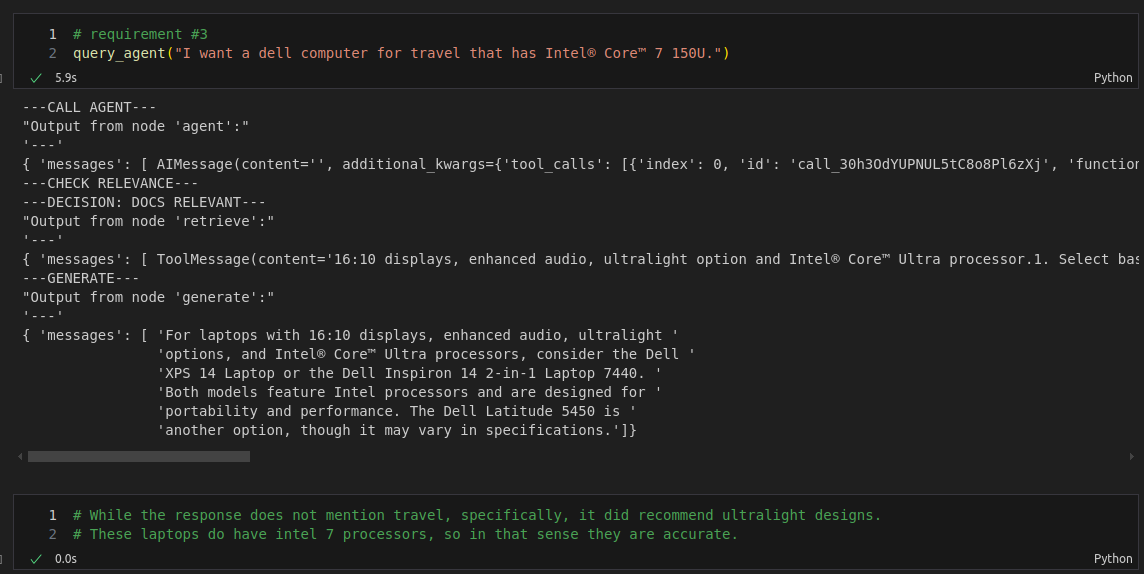
\includegraphics[width=1.0\linewidth]{q1.png}
\end{center}

The second query, \textit{`I want a dell computer that has Intel® Core™ Ultra 5 135U vPro® and has 512 GB SSD.'}, and its response are displayed below. It included specific requirements on the desired memory. The response addresses this but also includes other options that have different memory specifications. 

\begin{center}
    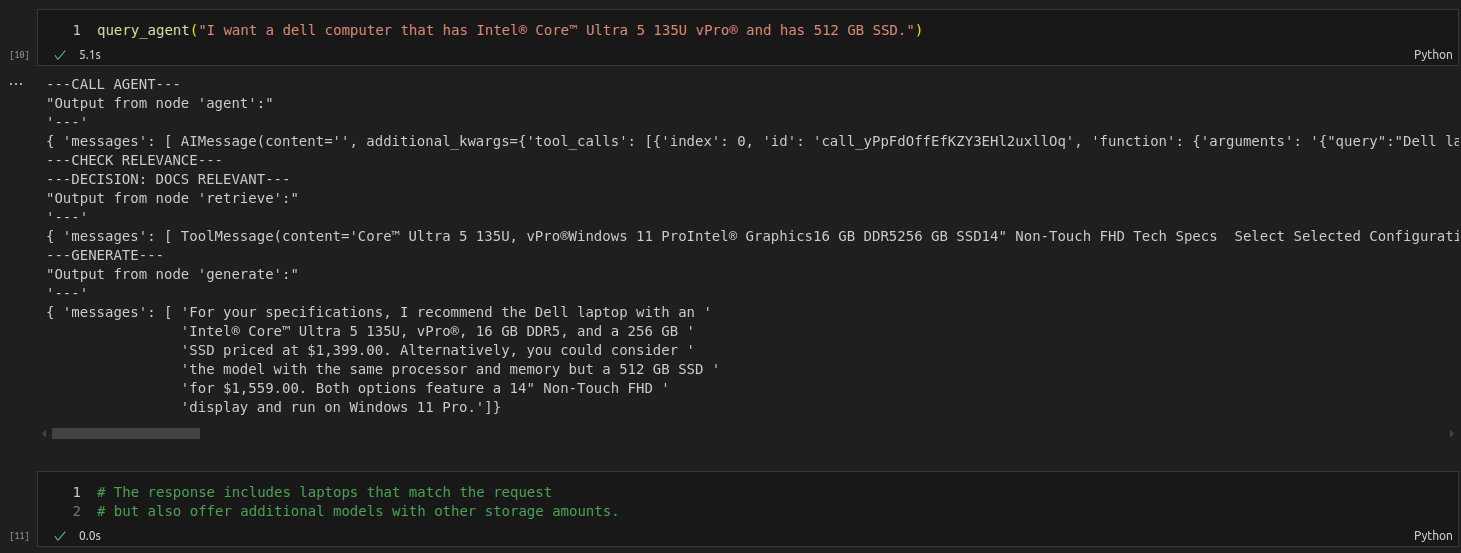
\includegraphics[width=1.0\linewidth]{q2.png}
\end{center}

The third query, \textit{`I want a dell computer that has Intel® Core™ Ultra 7 165U vPro® and 1 TB SSD'}, takes a similar approach- requesting a particular processor with a particular amount of storage.
The agent performs poorly on this query. The recommended laptop was wrong on both counts. The agent is not ensuring the requested specifications are being honored.

\begin{center}
    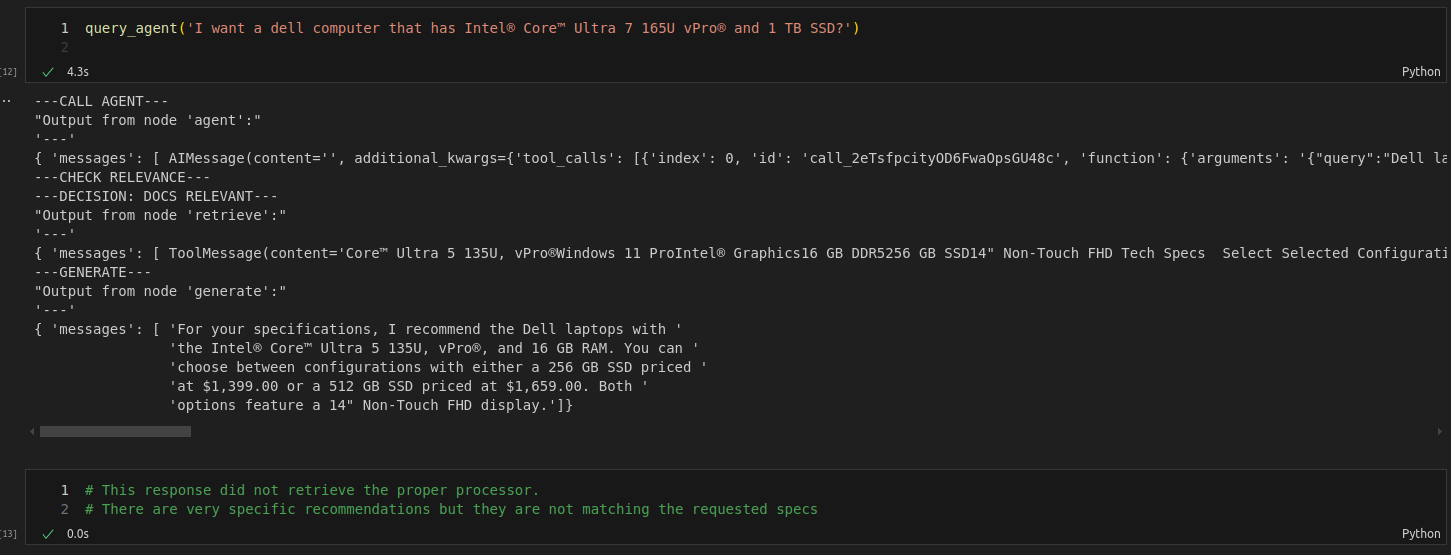
\includegraphics[width=1.0\linewidth]{q3.png}
\end{center}

The final query is \textit{`I want a light weight XPS computer with Intel® Core™ Ultra 7 165U vPro® and 1 TB SSD.'} It is very similar to the prior query however the agent handled it better. The recommended models are all `ultralight.'

\begin{center}
    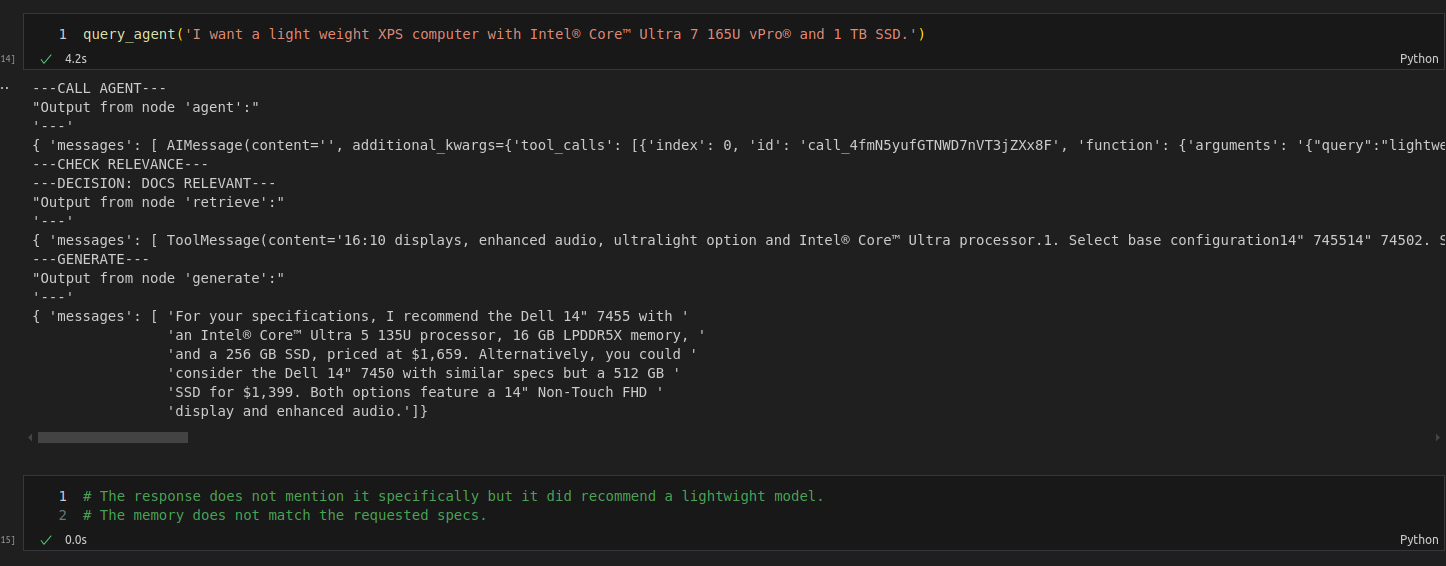
\includegraphics[width=1.0\linewidth]{q4.png}
\end{center}

In my experimentation I noticed the agent does better when the prompt is phrased as a question. To test this hypothesis I ran one additional query: \textit{`What laptop has the Intel 7 processor?'} The agent handles this one perfectly with a complete response that accurately and coherently addresses the prompt.

\begin{center}
    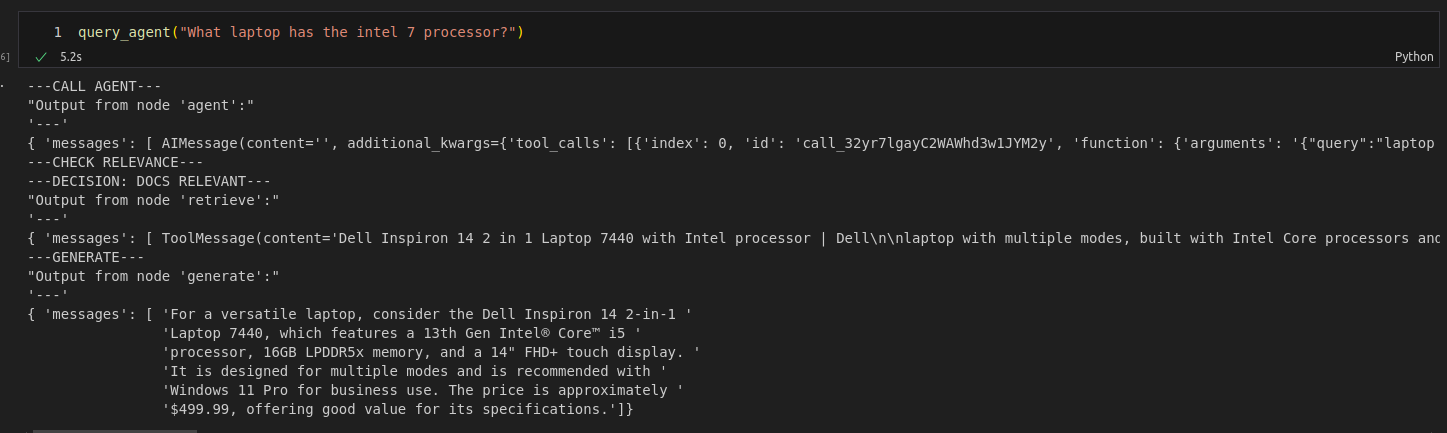
\includegraphics[width=1.0\linewidth]{q5.png}
\end{center}


\section*{Requirement 4: Response consistency}
\tab The experiments conducted in the assignment show that responses from the agent lack consistency. This is curious when we note the low (0.2) temperature we use when invoking the LLM. Running the same query over and over provides varied results. Sometimes the agent fails to see the question as relevant, sometimes the agent provides a very inaccurate response and sometimes the agent provides a suitable answer that addresses the prompt (directly or indirectly) with varying amounts of extraneous information. This is a focus for the proposed improvements to the agent listed below.

\section*{Requirement 5: Agent improvements}
\tab There are two primary issues that must be addressed. The first, is the agent failing to recommend laptops that meet the specifications in the prompt. Sometimes they are ignored, other times the recommendations are not limited to those specs. To improve this we can construct another node- recommendation vetting. This step can have the LLM evaluate the proposed response against the original human message. If the response does not meet the test the agent must circle back around and try again.

The second flaw that needs to be addressed is the lack of consistency. This might be mitigated by altering the way we preprocess the documents that are available for inclusion in the context. It may be advantageous to extract the specifications from the documents and store these along side the raw source material. Our experiment has suggested the agent performs well when simply listing the specs of a given model. The LLM could be leveraged to distill the components of each available model and, in turn, provide a clear manifest for subsequent queries.

\end{document}